%----------------------------------------------------------------------------------------
%	PACKAGES AND DOCUMENT CONFIGURATIONS
%----------------------------------------------------------------------------------------
\documentclass{article}

\usepackage{graphicx} 	% Required for the inclusion of images
\usepackage{natbib} 	% Required to change bibliography style to APA
\usepackage{amsmath} 	% Required for some math elements 
\usepackage{cases} 
\usepackage{array}
\usepackage{caption}
\usepackage{subcaption}

\usepackage{xcolor}
\usepackage{listings}
\usepackage{color}		 %red, green, blue, yellow, cyan, magenta, black, white
\usepackage{geometry}
\geometry{
a4paper,
total={170mm,257mm},
left=20mm,
top=20mm,
}
\setlength\parindent{0pt} % Removes all indentation from paragraphs

\definecolor{codegreen}{rgb}{0,0.6,0}
\definecolor{codegray}{rgb}{0.5,0.5,0.5}
\definecolor{codepurple}{rgb}{0.58,0,0.82}
\definecolor{backcolour}{rgb}{0.9,0.9,0.9}

\lstdefinestyle{mystyle}{
    %backgroundcolor=\color{backcolour},   
    frame=tb, 				% draw a frame at the top and bottom of the code block
    commentstyle=\color{codegreen},
    keywordstyle=\color{magenta},
    numberstyle=\tiny\color{codegray},
    stringstyle=\color{codepurple},
    basicstyle=\footnotesize,
    breakatwhitespace=false,         
    breaklines=true,                 
    captionpos=b,                    
    keepspaces=true,                 
    numbers=left,                    
    numbersep=5pt,                  
    showspaces=false,                
    showstringspaces=false,
    showtabs=false,                  
    tabsize=4
}
\lstset{style=mystyle}


%----------------------------------------------------------------------------------------
%	DOCUMENT INFORMATION
%----------------------------------------------------------------------------------------
\title{Artificial Intelligence in Control Engineering exercise}
\author{
	Lecturer: Dr.Pham Viet Cuong	\\
}
\date{October 08th, 2018}

\begin{document}
\maketitle 					% Insert the title, author and date

\begin{center}
	\begin{tabular}{l l}
	Group 9: \\
	Nguyen Chinh Thuy 	& 1513372	\\
	Nguyen Tan Phu		& 1512489	\\
	Le Van Hoang Phuong	& 1512579	\\
	Do Tieu Thien		& 1513172			\\
	Nguyen Tan Sy		& 1512872	\\
	Nguyen Van Qui		& 1512702
	\end{tabular}
\end{center}


%----------------------------------------------------------------------------------------
%	SECTION 1
%----------------------------------------------------------------------------------------
\section{Problem}
\textbf{Description:}

A robot operates in an environment where static points (landmarks) are known (coordinates). Using Particle Filter and Extended Kalman Filter, we control the robot to follow a defined path. Actually, the robot has a laser that can measure its relative position to landmarks. Some parameters are given as the following:\\

* Number of particles: Unlimited and denote as $M$.\\

* Number of steps: $N=625$.\\

* Control signal frequency: 40Hz.\\

* Defined path: $XTRUE = [xtrue_1, xtrue_2, ..., xtrue_N]$ of size [3xN], where $xtrue_i = [x_n, y_n, \phi_n]$.\\

* Landmark: $lm = [coord_1, coord_2, ..., coord_L]$ of size [2xL], where $coord_l = [x_l, y_l]$.\\

* Measurement: $Z$ of size [3x5xN], where $z_n = [z_1, z_2, z_3, z_4, z_5]$ of size [3x5] represents measured range at the time step $n$, in which $z_i = [r_i, b_i, idx_i]$.\\

* Control signal: $VG = [vg_1, vg_2, ..., vg_N]$ of size [2xN], where $vg_n = [v_n, g_n]$.\\

Due to thermal noise, measured values of velocity ($v$), steering angle ($g$), range ($r$), bearing angle ($b$) have errors. These errors have zero means and standard deviations of $\sigma_v=0.5m/s, \sigma_g=3^0, \sigma_r=0.2m, \sigma_b=2^0$, respectively. Data of $XTRUE$, $Z$, $lm$, and $VG$ is given the the file ``data20171107.m".\\

\textbf{Questions:}

a. Plot the defined path and controlled paths with 3 particles, namely maximum, median, and minimum important factor, using Particle Filter.

b. Compute the Root Mean Square error of the controlled paths to the defined path.

c. Repeat a and b using Extended Kalman Filter.


%----------------------------------------------------------------------------------------
%	SECTION 3
%----------------------------------------------------------------------------------------
\pagebreak
\section{Implementation}

\subsection{Particle Filter}

\subsubsection{Algorithm}
To solve the Paticle Filter problem, we implement follow below steps: \\
\begin{itemize}
	\item{Prediction} 
	\begin{itemize}
		\begin{subequations} 
		Process model:
		\begin{align}
			x_t = x_{t-1} + V_t\Delta{t}\cos\left({\theta_t + \varphi_{t-1}}\right) \\
			y_t = y_{t-1} + V_t\Delta{t}\cos\left({\theta_t + \varphi_{t-1}}\right) \\
			\varphi_t = \varphi_{t-1} + \dfrac{V_t\Delta{t}\sin{\theta_t}}{WB}
		\end{align}
		\end{subequations}
		\begin{subequations}
		Measurement model:
		\begin{align}
			r_t = \sqrt{{\left(x_t - x_L\right)}^2 + {\left(y_t - y_L\right)}^2}\\
			b_t = \arctan{\dfrac{y_t - y_L}{x_t - x_L}} + \varphi_t
		\end{align}
		\end{subequations}
		\item{Measurement model}
		\item{Implementing a loop with $M$ step which is numbers of particles}
		\item{Using process model and control signals $u_t$ in \textbf{VG} which are affected by thermal noise to calculate coordinate $x^{[m]}_t$ of robot.}
		\item{Combining coordinate of robot from above step and coordinate of landmarks in \textbf{lm} to calculate range $r_t$ and bearing angle $b_t$.}
		\item{Calculating importance factor $w^{[m]}_t$ depend on probability density function fomula with $\mu$ is matrix of expected range and bearing which are from \textbf{Z}.}
		\begin{align}
			f_x(x_1,x_2,...,x_N) = \dfrac{1}{\left(2\pi\right)^{\dfrac{N}{2}}\Vert\Sigma\Vert^{\dfrac{1}{2}}}exp\left(\dfrac{-1}{2}\left(x-\mu\right)^T\Sigma^{-1}\left(x-\mu\right)\right)
		\end{align}
	\end{itemize}
	\item{Selection}
	\begin{itemize}
		\item{Implementing a loop with $M$ step.}
		\item{Choosing a index in range $\left[1,M\right]$ for $x^{[m]}_t$ with probabilities $w^{[m]}_t$.}
	\end{itemize}
\end{itemize}

%\subsubsection{Python code}
%\lstinputlisting[language=Python]
%{../main.py}

%----------------------------------------------------------------------------------------
%	SECTION 4
%----------------------------------------------------------------------------------------
\subsubsection{Result} 
\begin{figure}[h!]
\centering
\begin{subfigure}[b]{0.8\linewidth}
	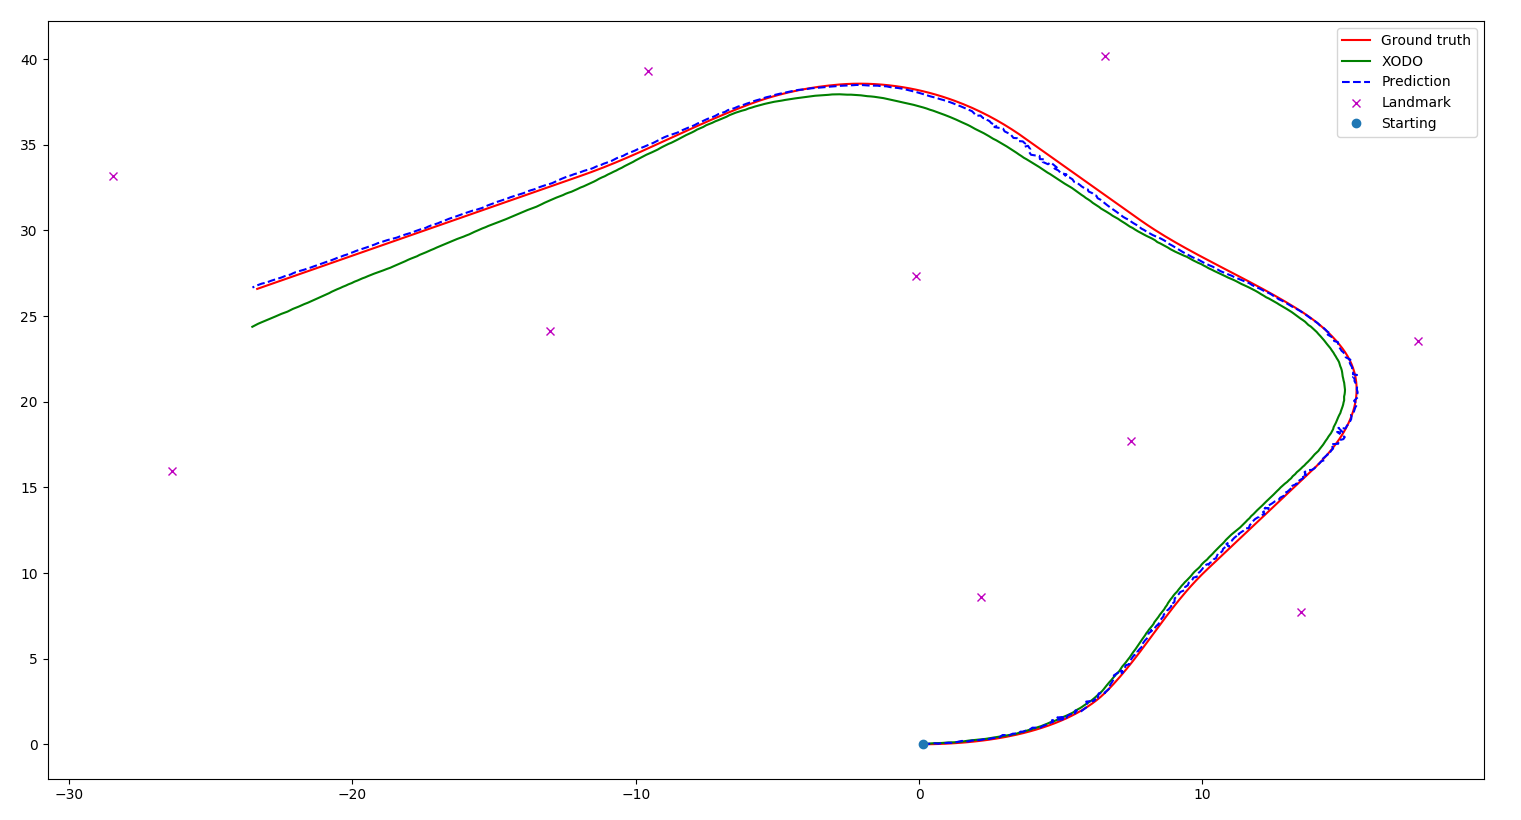
\includegraphics[width=\textwidth]{max.png}
	\caption{Trajectories with max $w_t$. $RMS = 11.289769$}\label{fig:image-1}
\end{subfigure}
\begin{subfigure}[b]{0.8\linewidth}
	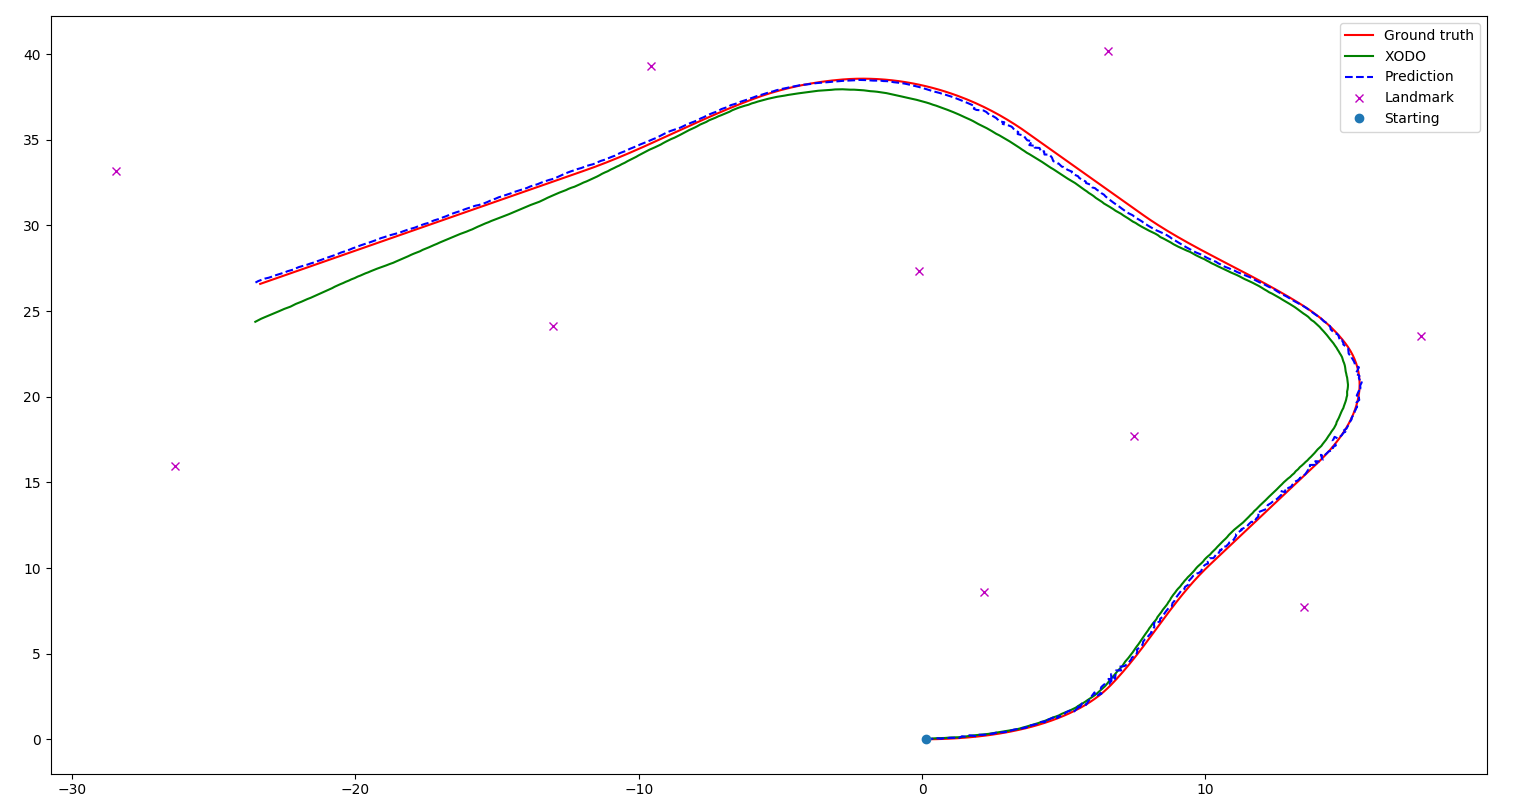
\includegraphics[width=\textwidth]{median.png}
	\caption{Trajectories with median $w_t$. $RMS = 11.428931$}\label{fig:image-2}
\end{subfigure}
\begin{subfigure}[b]{0.8\linewidth}
	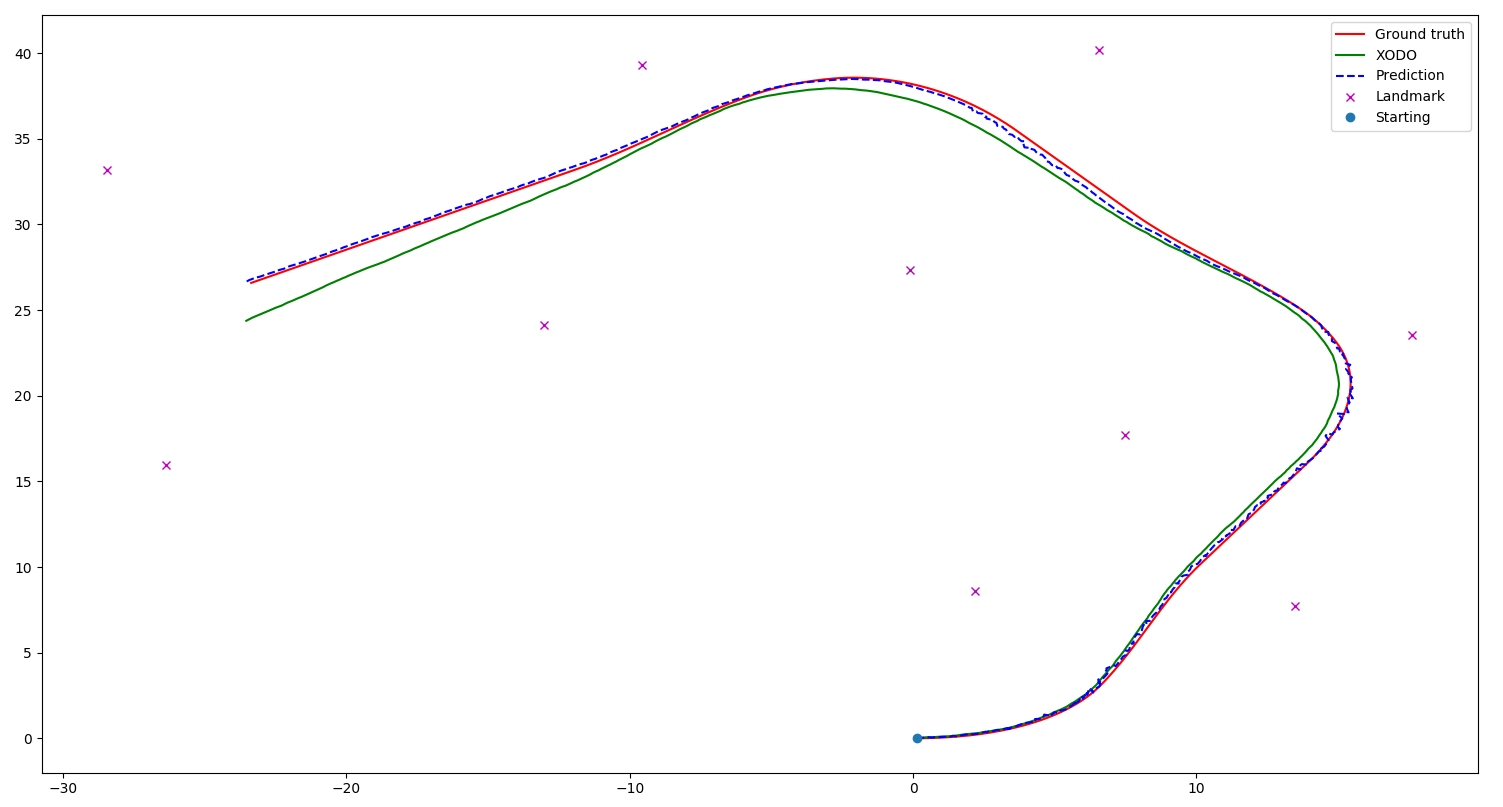
\includegraphics[width=\textwidth]{min.png}
	\caption{Trajectories with min $w_t$. $RMS = 11.475249$}\label{fig:image-3}
\end{subfigure}
\caption{Trajectories of Ground truth (XTRUE), XODO, Prediction and root mean square (RMS) of Prediction compared to Ground truth.}
\end{figure}


\textbf{Comments:}

\begin{itemize}
	\item{Overall, three trajectories of Prediction fits Ground truth with the same patterns. However, the best fit is belong to trajectoty with choosing max $w_t$, so the root mean square is smallest.} 
	\item{Line of XODO which is calculated from process model is different from Ground truth because of effect on range and bearing angle from thermal noise, while Prediction is calculated and chosen with importance factor $w_t$. That is the reason why line of Prediction is better than XODO.}
\end{itemize}


%----------------------------------------------------------------------------------------
%	SECTION 5
%----------------------------------------------------------------------------------------
\pagebreak

\subsection{Extended Kalman Filter}
\subsubsection{Algorithm}
\begin{itemize}
	\item{Extended Kalman Filter Overview: }	\\
The extended Kalman filter (EKF) calculates an approximation to the true belief. It
represents this approximation by a Gaussian distribution. The belief is merely an approximated form, not exact as the case in Kalman filters. The next-state probability and the measurement probability are governed by nonlinear functions.
\end{itemize}


\begin{figure}[!h]
    \centering
    \begin{subfigure}[b]{0.6\textwidth}
        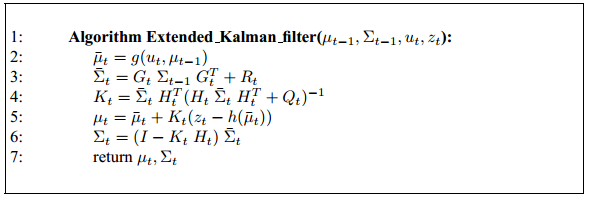
\includegraphics[width=\textwidth]{Algorithm-EKF.PNG}
        \label{fig:image-4}
    \end{subfigure}
\caption{Extended Kalman Filter Algorithm}
\end{figure}

\begin{itemize}
	\item{Design the system model:} 
	\begin{itemize}
		\begin{subequations} 
		Process model:
		\begin{align}
			x_t = x_{t-1} + V_t\Delta{t}\cos\left({\theta_t + \varphi_{t-1}}\right) \\
			y_t = y_{t-1} + V_t\Delta{t}\cos\left({\theta_t + \varphi_{t-1}}\right) \\
			\varphi_t = \varphi_{t-1} + \dfrac{V_t\Delta{t}\sin{\theta_t}}{WB}
		\end{align}
		\end{subequations}
		\begin{subequations} 
		We model system as a nonlinear model plus noise:
		\begin{align}
			x_t = g\left({u_t,x_{t-1}}\right)+ \epsilon_t 			
		\end{align}
		Calculate G by taking the Jacobian of g (nonlinear function):
	
		\begin{align*}
		G=
    		\begin{bmatrix}
        	1 & 0 & -R\cos\left({\theta}\right)+ R\cos\left({\theta+ \varphi}\right) \\
        	0 & 1 & -R\sin\left({\theta}\right)+ R\sin\left({\theta+ \varphi}\right) \\
        	0 & 0 & 1
    		\end{bmatrix}
		\end{align*}
		\end{subequations}

		\end{itemize}
\end{itemize}


\begin{itemize}
	\item{Design the measurement model:} 
	\begin{itemize}

		\begin{subequations}
		Measurement model:
		r(t) is range between state of robot and position of landmark. The sensor provides bearing relative to the orientation of the robot, we subtract the robot's orientation from the bearing to get the sensor reading b(t)
		\begin{align}
			z_t = h\left({x_t}\right)+ \delta_t 	\\		
			r_t = \sqrt{{\left(x_t - x_L\right)}^2 + {\left(y_t - y_L\right)}^2}\\
			b_t = \arctan{\dfrac{y_t - y_L}{x_t - x_L}} + \varphi_t
		\end{align}
		\end{subequations}
		\end{itemize}
\end{itemize}


%%----------------------------------------------------------------------------------------
%%	SECTION 6
%%----------------------------------------------------------------------------------------
%\pagebreak
%\subsubsection{Python code}
%\lstinputlisting[language=Python]
%{../EKF_final.py}

%----------------------------------------------------------------------------------------
%	SECTION 7
%----------------------------------------------------------------------------------------
\pagebreak
\subsubsection{Result} 
\begin{figure}[h!]
\centering
\begin{subfigure}[b]{0.8\linewidth}
	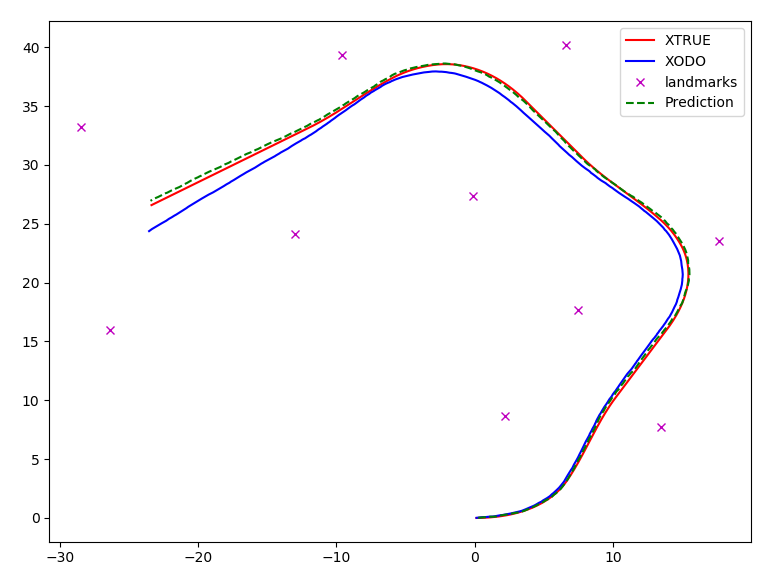
\includegraphics[width=\textwidth]{EKF.png}
	\caption{Root Mean Square $(RMS) = 26.201$}\label{fig:image-5}
\end{subfigure}
\caption{Position of lanmarks, path of Ground truth (XTRUE), XODO, Prediction(using EKF) and RMS.}
\end{figure}


\textbf{Comments:}

\begin{itemize}
	\item{The prediction result (the green dash line) is quite tight to the ground truth (the red line). This reveals that the Extended Kalman Filter is capable enough for controlling the robot to follow the defined path, despite of the approximation of the belief.} 
	\item{The value of RMS in the case of using Extended Kalman Filter is worse than using Particle Filter. This can be explained that the Extended Kalman Filter try to approximate the belief by a Gaussian distribution, this may lead to error which depends on how the belief form is closed to a Gaussian distribution. Meanwhile, the Particle Filter does not assume the belief can be approximated by any kind of normal distribution. It directly figure the belief regardless its form of distribution. Therefore, the result of the Particle Filter is more correct than one of the Extended Kalman Filter.}
	\item{Nevertheless, when carrying out an experiment to measure execution time between the Particle Filter and Extended Kalman Filter, we recognize that the runtime of the Extended Kalman Filter is much faster than of the Particle Filter (367ms comparing to 4905ms). This is due to the linear approximation of the Extended Kalman Filter. In fact, the process and measurement model is non-linear, which requires a complex computation. The Extended Kalman Filter, in this assignment, proves that its approximation of the non-linear models can reduce the computation time, but only endure a small error. Any way, its result can be accepted.}
\end{itemize}




\end{document}